\documentclass[12pt,titlepage]{article}
\usepackage[ngerman]{babel}
\usepackage[utf8]{inputenc}

\usepackage[autostyle=true,german=quotes]{csquotes}%NC: needed for babel

\usepackage[a4paper , lmargin = {2.5cm} , rmargin = {2.5cm} , tmargin =
{2cm} , bmargin = {2cm}]{geometry}

\usepackage[hyphens]{url}
\usepackage[linktocpage=true]{hyperref}

\usepackage{tabularx}

\usepackage{amsmath}
%\numberwithin{equation}{section}

% ### Bibliographical Stuff ###
% Use \textcite{} and \parencite{} with biblatex!
\usepackage[backend=biber,
    style=numeric-comp,%alphabetic-verb,
    sortlocale=de_DE,
    natbib=true,
    url=true, 
    doi=true,
    eprint=false]{biblatex}%NC: replaced bibtex by biber
\addbibresource{literatur.bib}%Dateiname für Quellen einfügen
\usepackage{ragged2e} %für bessere URL formatierung bei printbibliography 

%Bilder einbinden und auf der gleichen seite ein
%Fußnotenzitat einzufügen
%https://en.wikibooks.org/wiki/LaTeX/Importing_Graphics
\usepackage{graphicx}
\DeclareGraphicsExtensions{.pdf,.png,.jpg} %order of preference
\graphicspath{ {./images/} } %NC: Additional path to look for images in (placed higher up to support one location for multiple documents)
%\usepackage{float} %NC: Causes problems. deactivate this and the next
%\usepackage{afterpage} %need to use with: \af­ter­page{\clearpage} https://www.ctan.org/pkg/afterpage?lang=de

\interfootnotelinepenalty=99999 %Seitenumbruch einer Fußzeile verhindern

\usepackage{moreverb} %tabulator formatierung in verbatim umgebung

%Tables:
\newcolumntype{b}{X}
\newcolumntype{s}{>{\hsize=.5\hsize}X}

\newcommand{\bildcite}[6]{
     \begin{figure}[H]
         \includegraphics[width=\textwidth]{Bilder/#1}
         \caption[#2]{#2\footnotemark}
         \label{#3}
     \end{figure}
     \footnotetext{\cite[#6][#5]{#4}}
}

\newcommand{\bild}[3]{
     \begin{figure}[H]
         \includegraphics[width=\textwidth]{Bilder/#1}
         \caption{#2}
         \label{#3}
     \end{figure}
}

\renewcommand{\labelenumi}{\arabic{enumi}.}
\renewcommand{\labelenumii}{\arabic{enumi}.\arabic {enumii}}
\renewcommand{\labelenumiii}{\arabic{enumi}.\arabic{enumii}.\arabic{enumiii}}

\newcommand{\firstpages}{
    % \input{0_Deckblatt.tex}

     \newpage
     \tableofcontents{}
     \addtocontents{toc}{~\hfill\textbf{Seite}\par}

     \newpage
     \listoffigures

     \newpage
     \listoftables
     \newpage
}


\begin{document}
\title{\huge{Wirtschaftlichkeit von energieeffizienten Netzkonzepten} \\ \large{Projektbericht}} 
\author{Veronika Lawrence, Carmen Scheer, Nicholas Cariss, Maximilian Junker,\\ Christian Keck, Stefan Ludowicy, Dominik Schneider} 
\maketitle
\firstpages
%\twocolumn

%START HERE
\section{Einleitung}
Hier muss auch was stehen, oder? 
In der vorliegenden Arbeit...
Sollten wir evtl die Unterkapitel-Aufteilung weg lassen?
%TODO Klimalwandel, CO2, 
%TODO Potential alternativer Energiequellen
% siehe auch Todoist Kommentar
%TODO Dominik


\section{Stand der Forschung} \label{SdF}
Definition Wirtschaftlichkeit, Carriernetz
Betriebskosten, Wirtschaftlichkeit, etc.
CAPEX OPEX
Wirtschaftlichkeit
Definieren
Wir betrachten einen Teil der Betriebskosten, nämlich: .....
% Evtl. die Sachen zu Wirtschaftlichkeit mit einem Hinweis, dass wir uns auf einen Teil, nämlich die Betriebskosten beschränken, in entweder Problemstellung oder Methodik

\subsection{Carrier-Netzwerke} 

%Text übernommen aus dem Exposé, muss noch ausformuliert werden - VL
%
%TODO: Mehr beschreiben, was schon getan wurde
%TODO: Verschiedene Methoden gegenüberstellen

Gegenstand der Projektarbeit bildet ein hinsichtlich der Energieeffizienz und Wirtschaftlichkeit zu optimierendes Carrier-Netzwerk.

Unter einem Carrier "`versteht man […] eine Gesellschaft, die mindestens drei Übertra\-gungs\-wege betreibt, die über eine Vermittlungsstelle miteinander verbunden sein müssen"' (aus: \cite{carrier}). Ein Carrier-Netzwerk stellt somit physikalische Transportwege und -verfahren zur Verfügung und bildet die Grundlage für sogenannte Value Added Services von Providern, welche auf den Carrier-Diensten aufsetzen \cite{fassnacht}. "`Bei den TK-Transportwegen unterscheidet man leitergebundene Verbindungen auf der Basis von Kupferkabeln oder Lichtwellenleitern sowie Funkverbindungen wie Satellitenverbindungen, Richtfunkstrecken und Rundfunkverbindungen"' (Aus: Ebd.).%TODO: Zitat korrigieren

Somit umfasst ein Carrier-Netzwerk nicht nur das physikalische Backbone-Netz, sondern auch das Zugangs- und Aggregationsnetzwerk. Im Rahmen des Projektes entfällt die Betrachtung der Optimierungspotentiale des Zugangsnetzes zugunsten einer aus\-führ\-lich\-eren Simulation von wirtschaftlichen und energieeffizienten Netzkonzepten im Backbone- und Aggregationsnetzwerk. So bildet der Broadband Network Gateway (BNG) die niedrigste Netzelementebene. Multi-Service Access Nodes (MSAN), Digital Subscriber Line Access Multiplexer (DSLAM), enhanced NodeBs (eNodeB) und weitere Netzelemente der nächsttieferen Hierarchiestufe fallen somit aus der Betrachtung.
\subsection{Möglichkeiten der Energieeinsparung in Netzwerken}
%Evtl mit dem nächsten Subchapter zusammenlegen? Hier nicht schreiben über unsere Simulation. Es geht nur darum, was andere schon erforscht haben.
Um den Energieverbrauch im Carrier-Netzwerk berechnen zu können, bedarf es an Werten der im Backbone verwendeten Netzkomponenten. Innerhalb der Simulation wird für die Berechnung des Gesamtverbrauchs auf die definierten Werte zurückgegriffen, die in einer Datenbank gespeichert sind. Ziel dieser Arbeit ist die Simulation und Berechnung des gesamtheitlichen Energieverbrauchs. Deshalb verwendet die Berechnung die von den beiden Wissenschaftler Ward Van Heddeghem und Filip Idzikowski in ihrer Veröffentlichung \cite{vanhedde} zusammengetragenen Werte. Die Quelle beinhaltet zum einen das analytische Model der Berechnung und zum anderen ein Datenblatt \cite{vanhsheet} des Energieverbrauchs der unterschiedlichen Hersteller. Das Datenblatt gliedert die Geräte nach den Unterschiedlichen Layer IP/MPLS, Ethernet, OTN, WDM - (OSI-Layer: 3-2-1-1). Zu beachten ist beim Verwenden der Werte, dass es sich um Werte unter typischen Lastbedingungen handelt, die sich nach der Kapazität der Komponente richtet und nicht nach dem aktuellen Durchsatz. Des Weiteren geben die Werte nur dein Stromverbrauch für den Betrieb an, ein Verbrauch für Kühlung o.Ä. ist nicht enthalten.
Der Gesamtverbrauch des Core-Networks ergibt sich aus der Summe alle Verbrauche der einzelnen Schichten. 

\begin{equation}
P_{core} = P_{ip} + P_{ethernet} + P_{otn} + P_{wdm}
\end{equation}


\subsection{Energie-effiziente Technologien}
Der aktuelle Stand der Forschung bietet verschiedene Konzepte und Technologien für das Einsparen von Energie in Carrier-Netzen. In dieser Arbeit sollen ausgewählte Konzepte und Technologien genutzt werden, um die Wirtschaftlichkeit von energieeffizienten Netzen zu analysieren. Betrachtet wurden im Rahmen der Literaturrecherche die folgenden Konzepte und Technologien: 

Das erste Konzept sieht eine Vereinfachung des Netzes vor, welche durch eine geographische Aufteilung des Netzes in Submodale (Global - Kontinental - National - Regional - Zugang) erfolgen kann \cite{aleksic2014}.

Das zweite Konzept befasst sich mit der dynamischen Abschaltung unterlasteter Netzkomponenten. Tageszeitabhängige Schwankungen des Traffics in Netzen ermöglichen eine individuelle und dynamische Abschaltung von Switches und Links unter der Be\-rück\-sich\-ti\-gung der QoS-Bedingungen \cite{aleksic2013}. Dabei werden Algorithmen zur Identifikation von individuell abschaltbaren Links verwendet \cite{fisher}.

Bei den Technologien beschränkt sich diese Arbeit auf optische leitungsvermittelnde Switche und das Hybrid Optical Switching (HOS). Optische leitungsvermittelnde Switche basieren auf mikro-elektromechanischen Systemen, die die geringste Menge an Energie benötigen und eine hohe Portanzahl besitzen. Das Hybrid Optical Switching verwendet eine Kombination aus optischen und elektronischen Netzknoten, die optische Leitungen, Bursts, und Pakete effizient Switches können. Durch die Kombination von langsamen und schnellen Switches, können Wellenlängenbereiche dynamisch zwischen zwei Switches geändert werden. Das temporäre Abschalten von ungenutzten Ports des schnellen Switches ermöglicht eine Energieeinsparung.  \cite{aleksic2013}

\section{Problemstellung}
Wie oben beschrieben existieren bereits einige Möglichkeiten, den Energieverbrauch in Carrier-Netzwerken zu senken. Allerdings werden diese Möglichkeiten noch nicht umfänglich in realen Netzwerken umgesetzt. Ein denkbarer Grund für diesen Rückstand realer Backbone-Netze sind wirtschaftliche Bedenken der Netzbetreiber. Im Folgenden wird die Motivation für Netzbetreiber beschrieben, den Energieverbrauch ihrer Netze stärker zu berücksichtigen, sowie die Ziele dieser Arbeit.
%citation needed!

\subsection{Motivation}
Obwohl der Stromverbrauch der OECD-Staaten seit mehreren Jahren stagniert oder sogar leicht zurück geht, wachsen die globalen Verbräuche weiter an (vgl. Abbildung \ref{fig:Strom_Sektor}). Dies kann vor allem auf  Schwellenländer zurückgeführt werden, die in kurzer Zeit ein rasantes wirtschaftliches Wachstum erleben.

\begin{figure}[!ht]
	\centering
	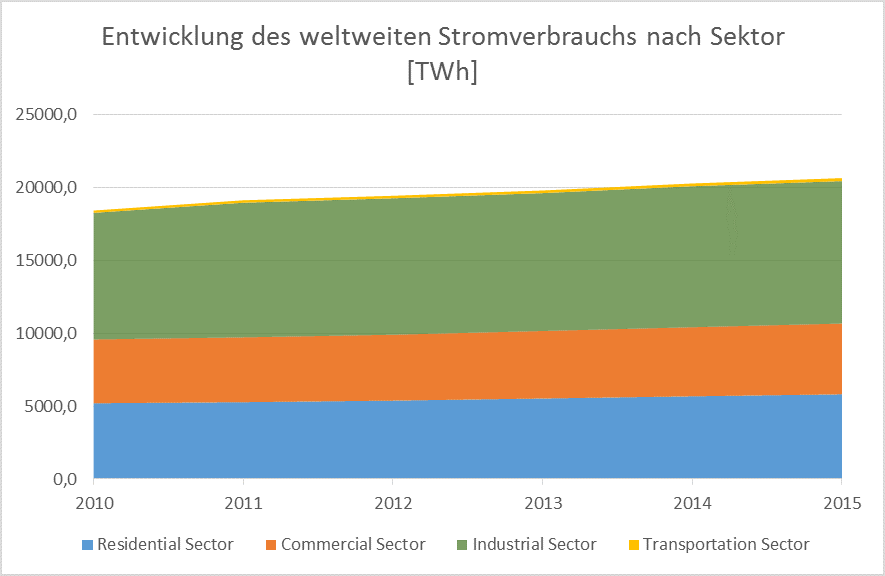
\includegraphics[width=0.8\textwidth]{Anteil_Strom_Sektor}
	\caption{Weltweiter Stromverbrauch nach Sektoren, basierend auf \cite{bibid}}
	\label{fig:Strom_Sektor}
\end{figure}
Da aller Bemühungen zum Trotz die fossilen Energieträger Erdöl, Kohle und Erdgas weiterhin ca. 81\% der weltweiten Energieerzeugung ausmachen \cite{statista} und diese Ressourcen nicht regenerierbar sind, sind langfristig steigende Energiekosten (\cite{iea2015}, S. 40f) ein großes Risiko für ICT-Provider weltweit, die insgesamt mit steigenden Kosten zu kämpfen haben.

Steigende Energiekosten für sich genommen wären schon ein starkes Argument, Netze effizienter zu gestalten.  Der Effekt der Kosten wird allerdings potenziert durch den Fakt, dass der Stromverbrauch von ICT von 2007-2012 stärker gewachsen ist als der globale Stromverbrauch (vgl. \cite{vanHeggedhem} S.9). Schon 2012 betrug der Anteil von ICT am globalen Stromverbrauch etwa 5\% (s. Abbildung \ref{fig:ICT_Strom}) 

\begin{figure}[!ht]
	\centering
	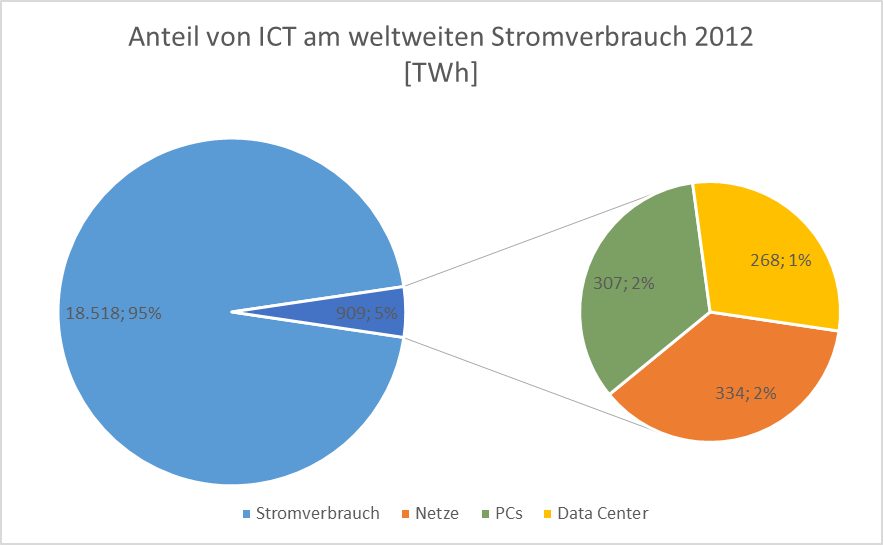
\includegraphics[width=0.8\textwidth]{Anteil_ICT_Strom}
	\caption{Anteil von ICT am weltweiten Stromverbrauch, basierend auf \cite{bibid} und \cite{bibid}}
	\label{fig:ICT_Strom}
\end{figure}

Seit dem ist der Anteil der Bevölkerung weltweit, der das Internet verwendet, von 20,6\% (2007) auf 43,4\% (2015) gestiegen \cite{itu}. Dieses Wachstum wird sich in der nächsten Zukunft nicht verlangsamen. Weiterhin sorgen steigende Datenvolumen pro Nutzer für eine wachsende Netzlast. Welchen Effekt die Industrie 4.0 und das Internet of Things auf die Netze weltweit haben werden, lässt sich momentan  noch nicht abschätzen. Eins jedoch steht fest: Das Netz der Zukunft wird mehr Daten zu bewältigen haben als jemals zuvor.
%evtl. nach oben ziehen als 1. Absatz für Problemstellung

\subsection{Ziele}
Das Ziel der vorliegenden Arbeit ist es, abzuschätzen, wie viel Energie bzw. Kosten  durch Verwendung energieeffizienter Technologien eingespart werden können.

Zur Erreichung dieses Ziels ist zum einen eine Literaturrecherche zu den bestehenden Technologien nötig, die es ermöglichen, den Energieverbrauch von Netzen zu senken. Die Ergebnisse dieser Literaturrecherche befinden sich in Kapitel \ref{SdF}.

Es soll eine Software entwickelt werden, die es ermöglicht, zwei hypothetische Netze miteinander zu vergleichen, zum einen ein konventionelles Netz, wie es heutzutage Stand der Technik ist, zum anderen ein energieeffizientes Netz, das die vorhandenen Technologien und Konzepte zur Effizienzsteigerung sinnvoll einsetzt. Anhand des abgeschätzten Energieverbrauchs der beiden Netze wird das Energiesparpotenzial sowie die möglichen Kosteneinsparungen durch den Betrieb des energieeffizienten Netzes ausgegeben. Die Ergebnisse der Softwareentwicklung sowie die Abschätzung des Energieverbrauchs befinden sich in Kapitel \ref{Ergebnisse}.

Die Softwarelösung wird als objektorientierte Java Desktop Anwendung mit einer Einteilung der Klassen in die drei Bereiche Model, View und Controller implementiert.

Der Prozess der Softwareentwicklung soll nach dem Wasserfallmodell ablaufen. Die Programmaufteilung und geforderte Funktionen sind bereits vor der Implementierung hinreichend bekannt, so dass die Anwendung eines agilen Entwicklungsmodells hier keine entscheidenden Vorteile bietet. Das genaue Vorgehen in der Softwareentwicklung wird im folgenden Kapitel erläutert.

\section{Vorgehen}

\subsection{Modellierung}
Zwei Netze modelliert (Quellen), um sie gegenüberstellen zu können. Techniken aus Kapitel "Energieeffiziente Technologien" eingesetzt.
Aufgrund der Recherche ist Simulation nötig.

\subsection{Softwareentwicklung}

Anforderungen an eine mögliche Simulationssoftware erarbeitet
Entscheidung/Festlegung Entwicklungmodell / Technologiestack / Systemlandschaft, weil....
Start Softwareentwicklung
	- Requirements
	- Spezifikation
	- Design
Implementierung
\subsection{Entwicklung des Routing-Algorithmus}
Zur Simulation des Netzwerkes, der Lastverteilung und des elektrischen Stromverbrauches des Netzwerkes ist ein iteratives Berechnen für einzelne Zeitabschnitte abhängig von der Netzlast, des Traffic-Ursprungs und des Traffic-Ziels notwendig. Grundlegend ist das Ziel, für jeden Zeitabschnitt die beste erzielbare Lösung zur stromsparenden Bewältigung (Durchleitung) des Traffics zu berechnen. Über die Dauer eines Zeitabschnittes (einer Iteration) bleiben die Routing-Entscheidungen und die Wahl der abzuschaltenden Hardware gleich. Diese werden je Iteration initial einmal berechnet. Durch die Anpassung der Iterationsdauer und der dazu passenden Anpassung der Netzlast-Daten lässt sich ein genaueres, verfeinertes Modell durchrechnen, so dass ein realistischeres Resultat zu erwarten ist.
\begin{figure}[!h]
	\centering
	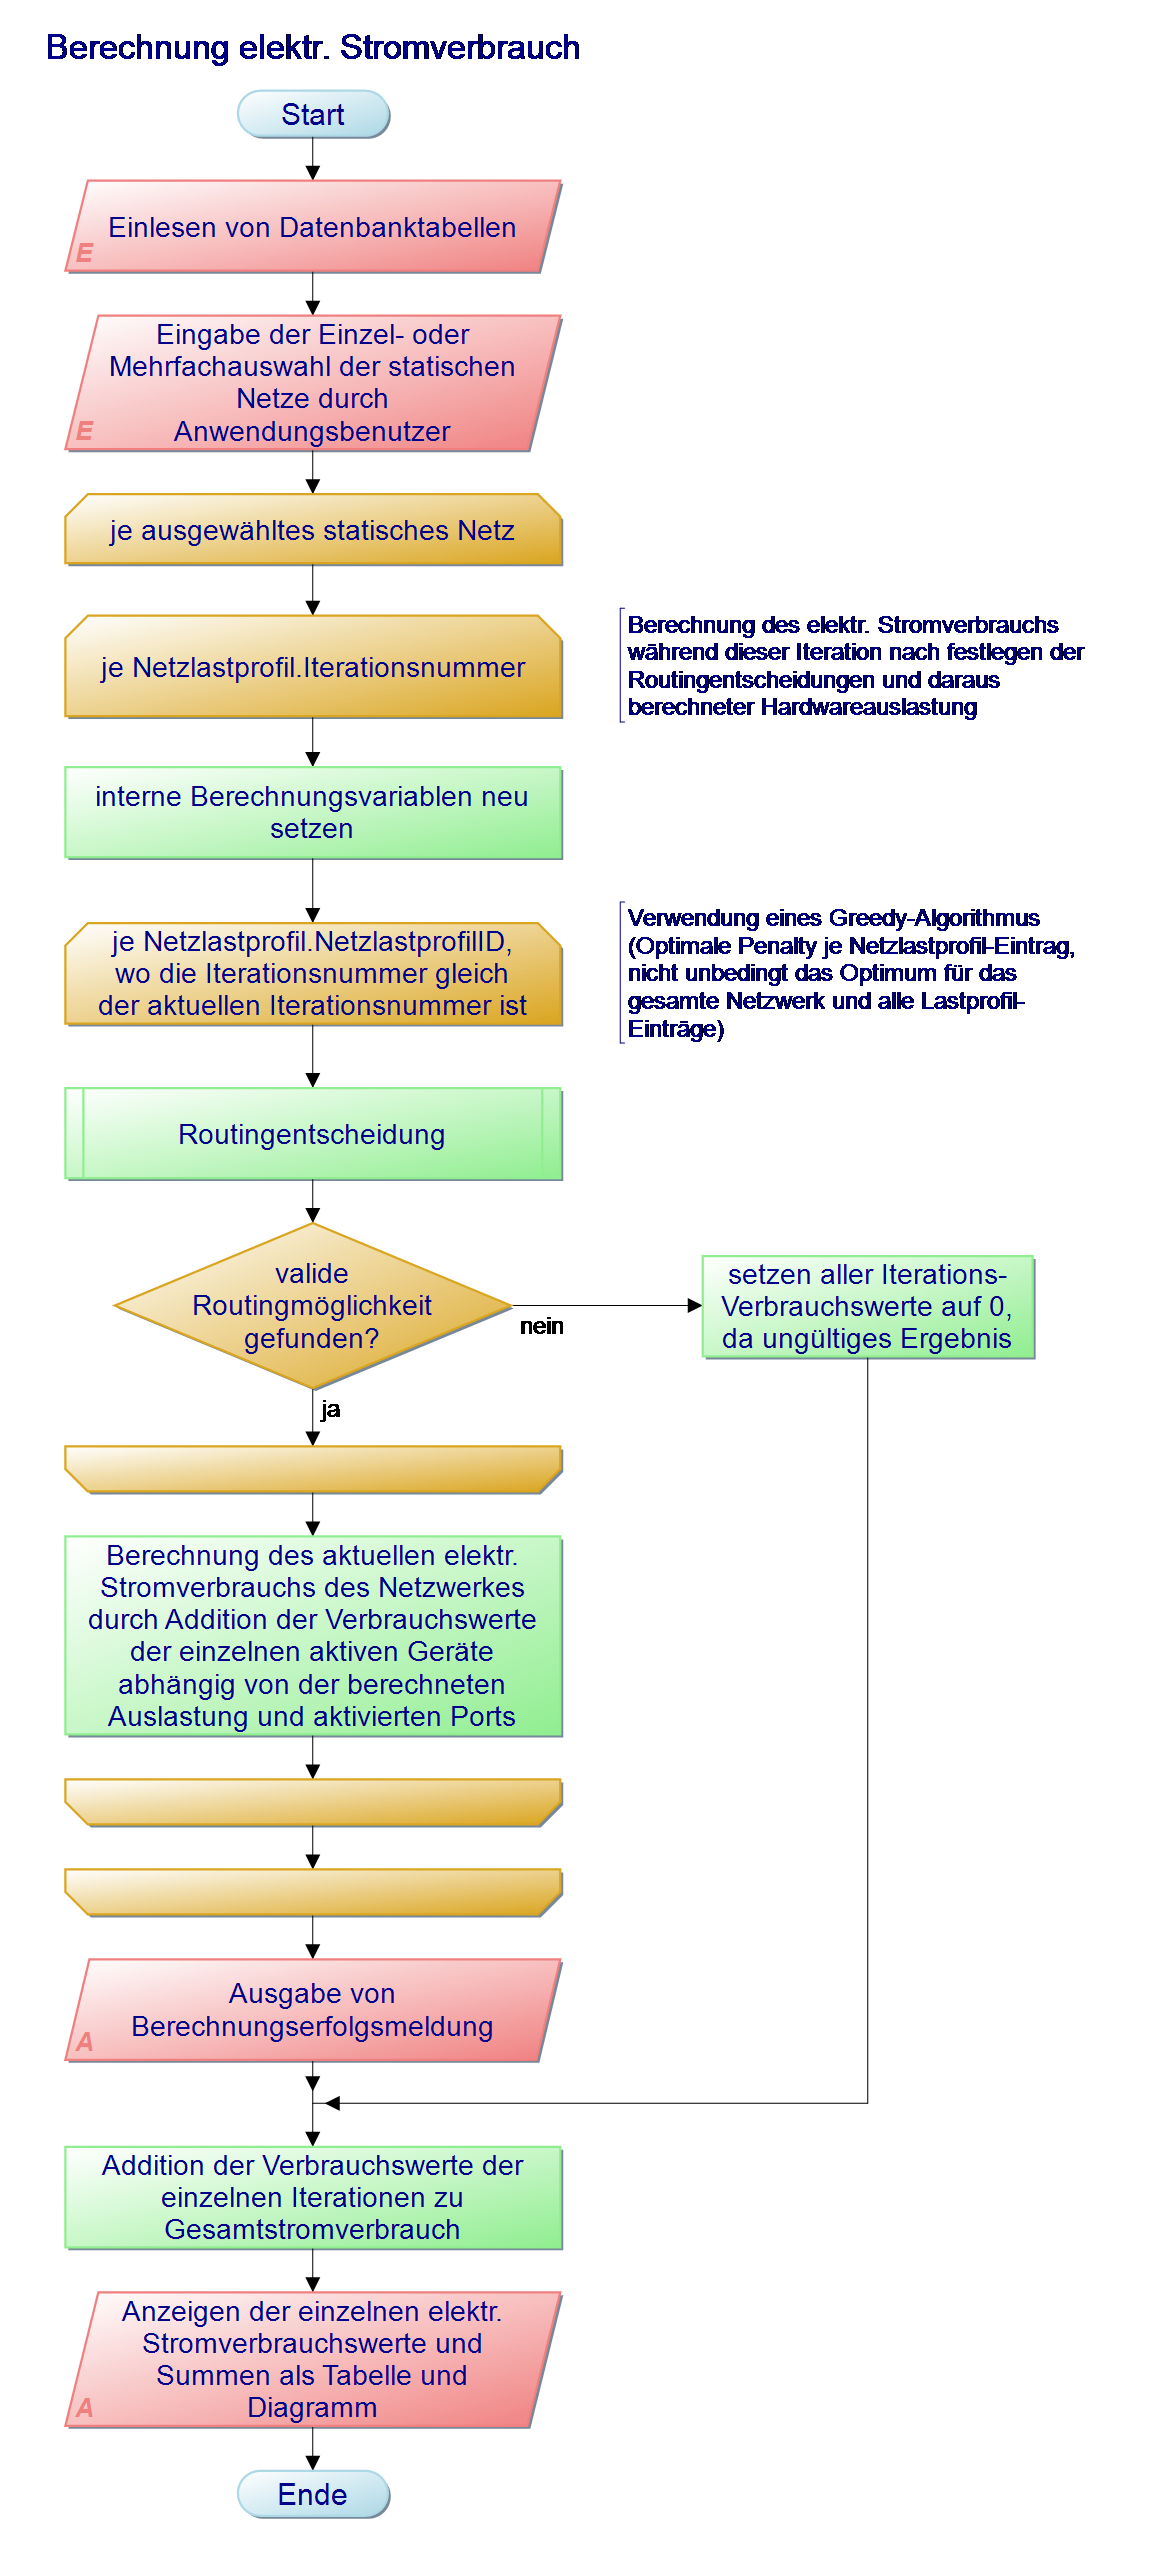
\includegraphics[width=0.6\textwidth]{1Berechnung_elektr_Stromverbrauch}
	\caption{Programmablaufplan zur Anwendungslogik}
	\label{fig:1Berechnung_elektr_Stromverbrauch}
\end{figure}

Um zu entscheiden, welches Routing für die einzelnen Netzlastprofil-Einträge je Iteration am "besten" ist, wird je mögliche Route eine dynamische Penalty (Kosten-Faktor) berechnet. Anschließend wird für das Netzlastprofil die Route mit der niedrigsten errechneten Penalty, welche die Datendurchsatzgrenzen der Hardware und somit der einzelnen Verbindungen nicht überschreiten, als beste Route angenommen. Um eine schnelle praktische Ausführungszeit zu erreichen beinhaltet dieser Algorithmus "Intelligenz" um schlechte Routen frühzeitig zu ignorieren und zum Beispiel Schleifenbildung zu verhindern.

\begin{figure}[!h]
	\centering
	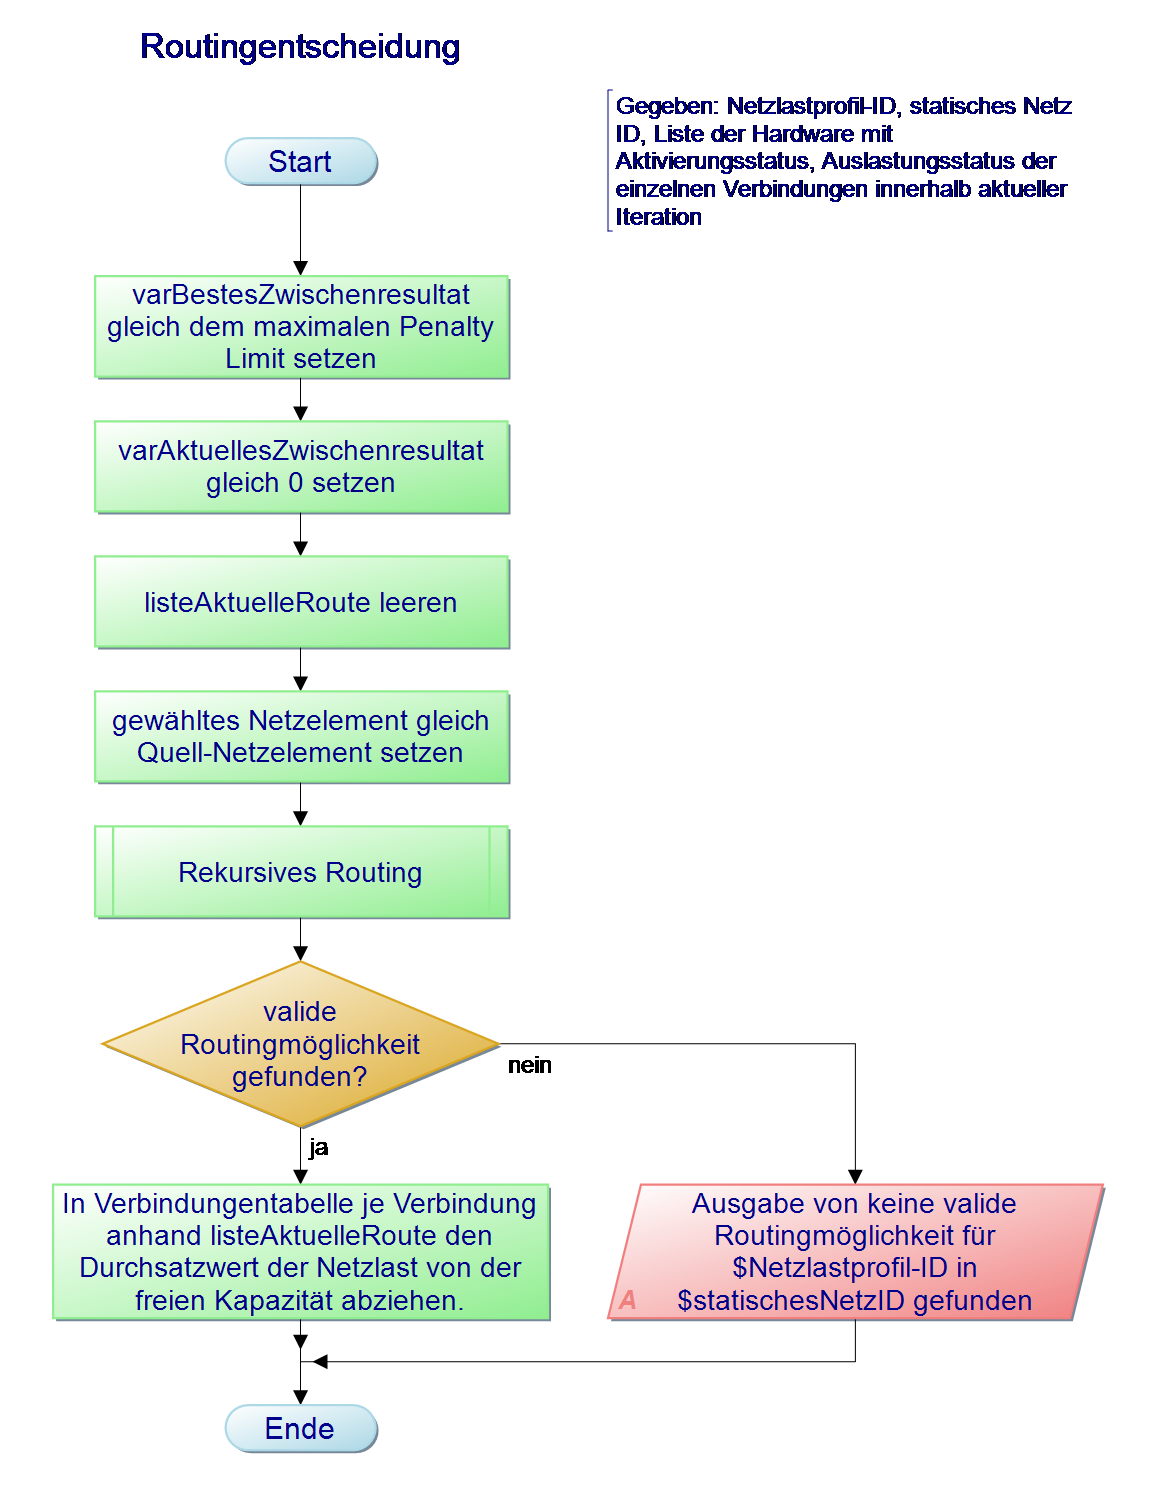
\includegraphics[width=0.6\textwidth]{2Routingentscheidung}
	\caption{Programmablaufplan zum übergreifenden Anteil des Routing-Algorithmus}
	\label{fig:2Routingentscheidung}
\end{figure}

Da die zur Verbindungsbewertung verwendete Penalty mehreren Faktoren wie Latenz, elektr. Stromverbrauch, Kapazität der Verbindung und auch An-/Aus-Status der Hardware berücksichtigen muss, und diese einzelnen Faktoren je nach Verwendungszweck des Netzes unterschiedliche Gewichtung haben, müssen die einzelnen Anteile mit vom Anwender der Simulationssoftware festgelegten Gewichtungsfaktoren multipliziert werden. Damit kann der Nutzer die Netzsimulation auf seine Anforderungen ansatzweise anpassen.

\begin{figure}[!h]
	\centering
	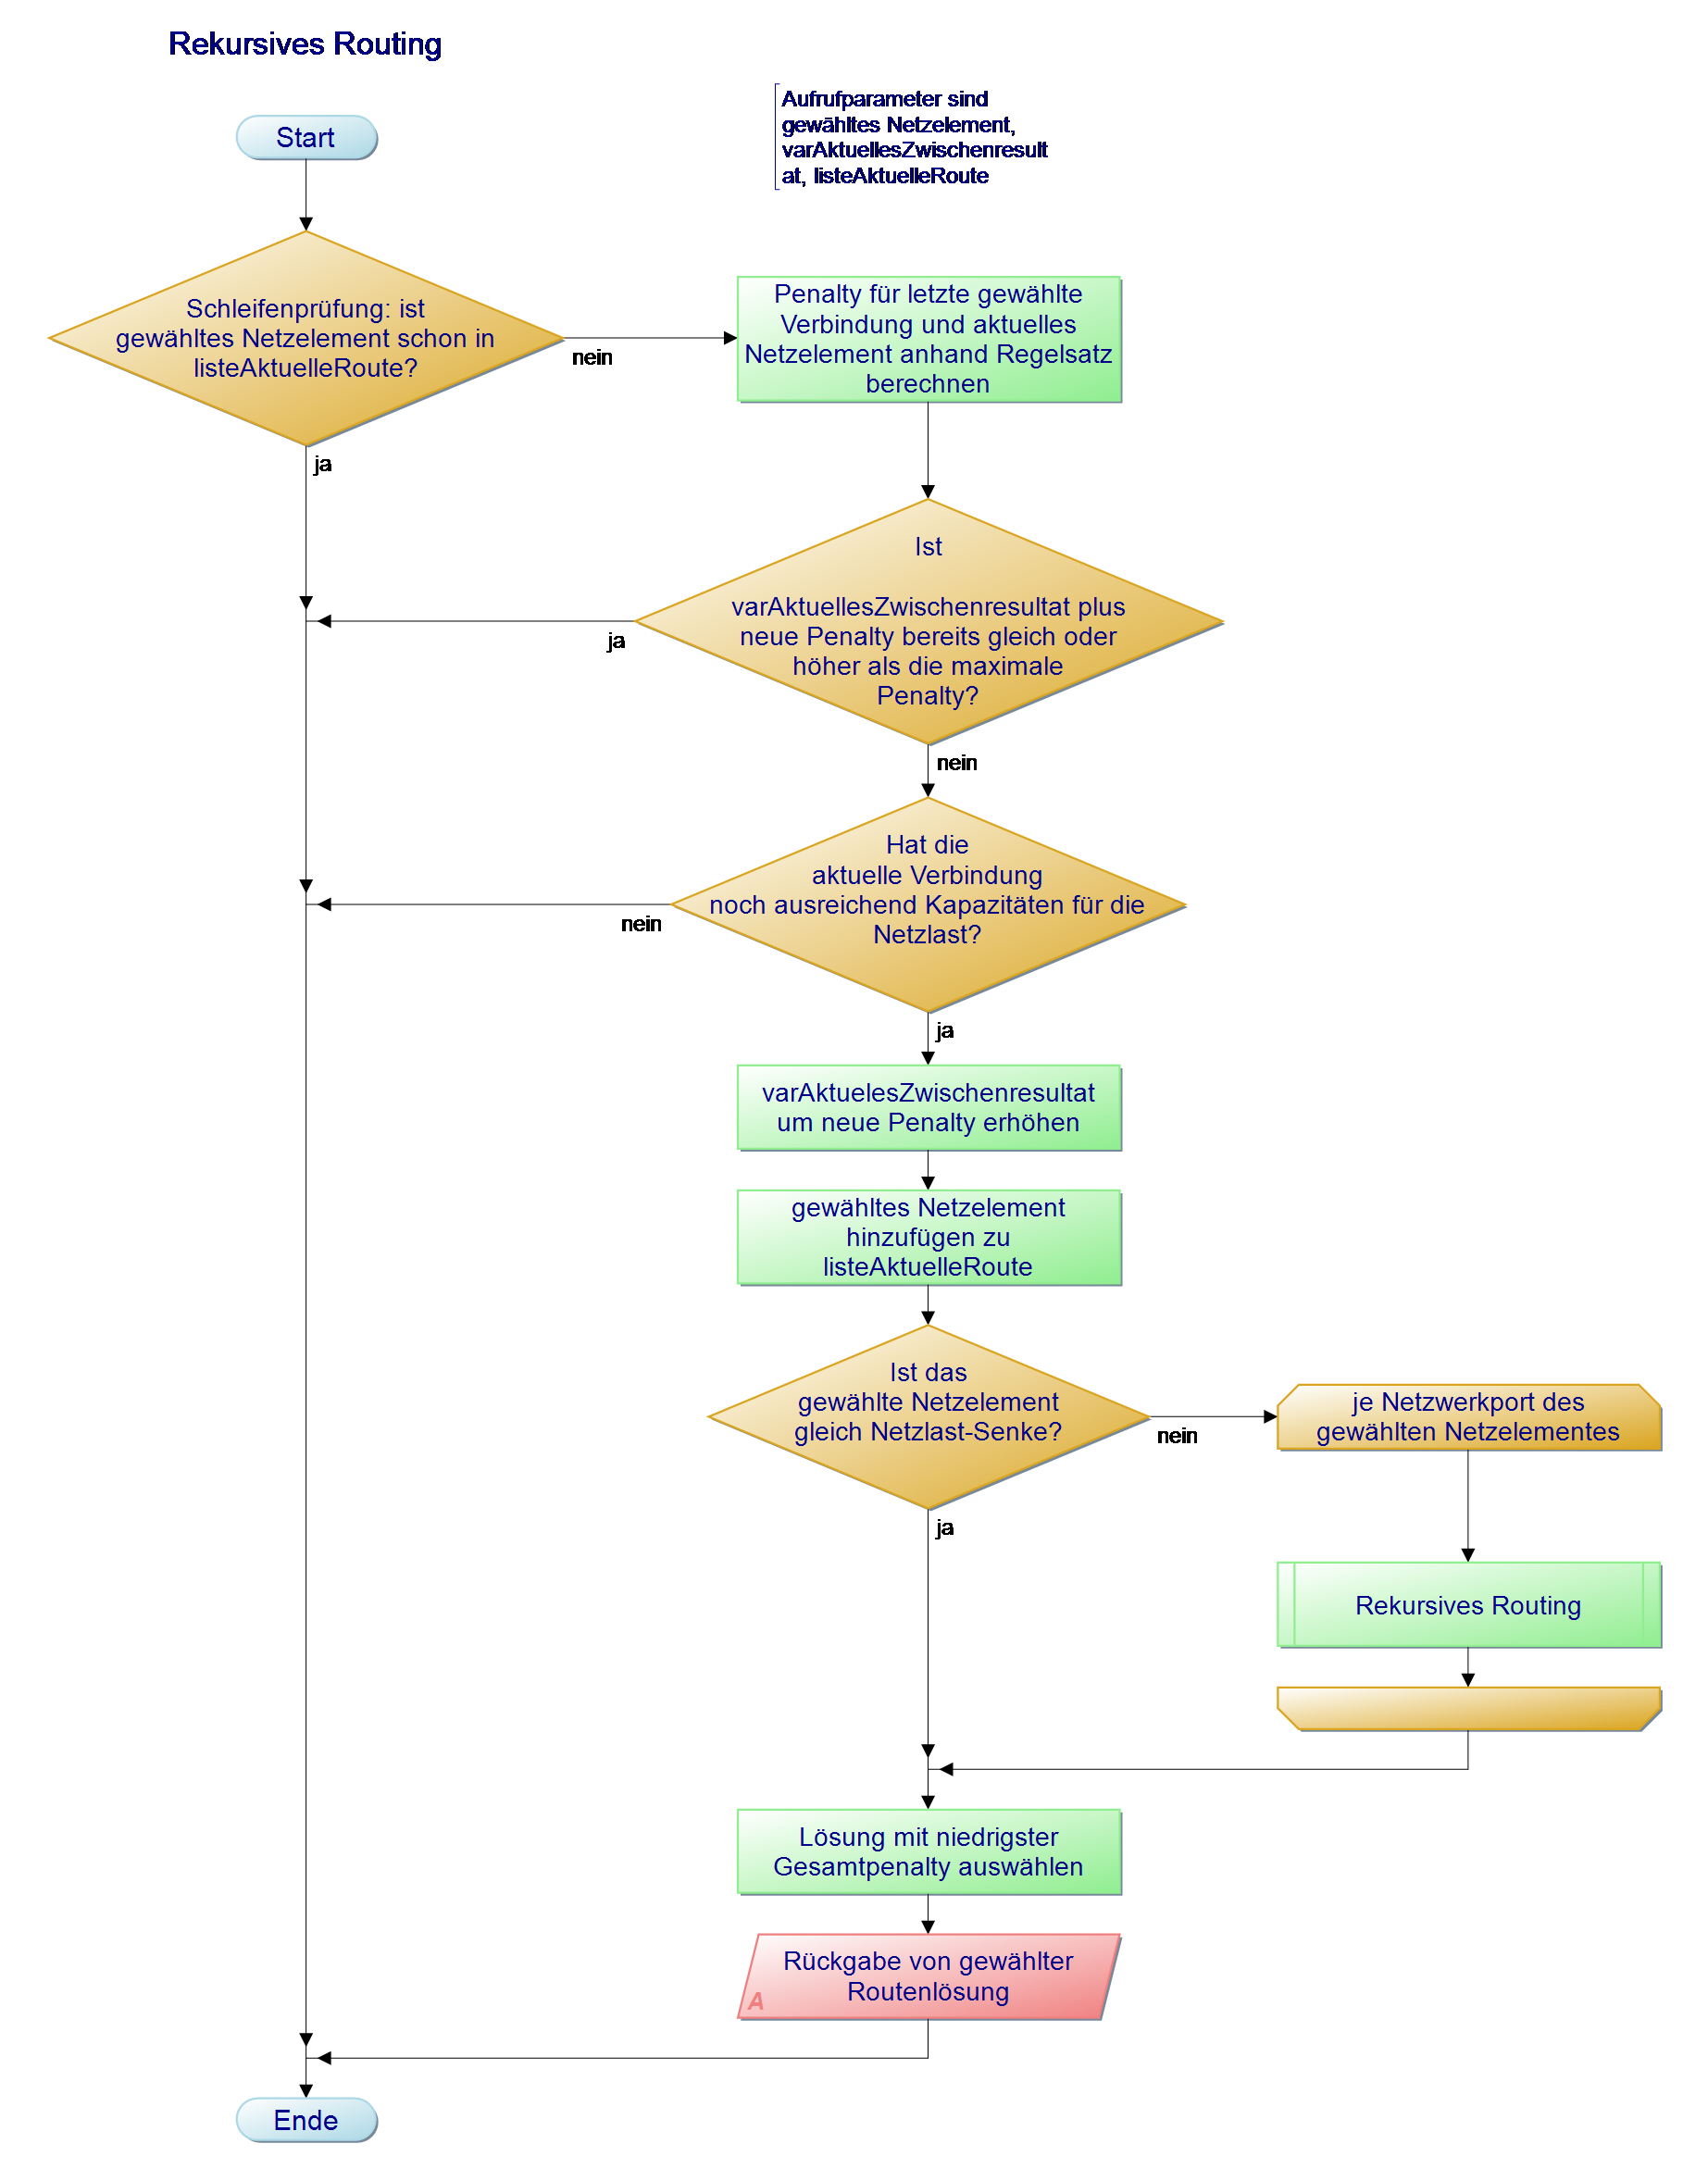
\includegraphics[width=0.6\textwidth]{3Rekursives_Routing}
	\caption{Rekursiver Anteil des Routing-Algorithmus}
	\label{fig:3Rekursives_Routing}
\end{figure}

Alles in allem ist ein Regelsatz zur Penaltyberechnung je Iteration notwendig, an Hand welchem die Algorithmus-Implementierung jeweils versucht das lokale Optimum zum Routingproblem als Lösung zu finden.
Der folgende Regelsatz stellte sich beim logischen durchspielen einer solchen Simulation als Grundlage heraus:
\begin{itemize}
\item Zum Anfang jeder neuen Iterations-Zeitphase sind alle Geräte und alle Ports soweit diese dies unterstützten ausgeschaltet
\item Das Aktivieren eines Devices kostet Penalty (hoch)
\item Das Aktivieren eines Ports kostet Penalty (niedrig)
\item Das Ausschalten des Port-Energiesparmodus kostet keine Penalty, um vermeidbares aktivieren anderer Hardware / Ports zu vermeiden. Energiesparmodus-Capability zählt lediglich zur Berechnung des Stromverbrauchs.
\item Um niedrige Paketlaufzeiten durch das Netz sicherzustellen, kostet jeder Hop / genutzte Verbindung eine weitere Penalty (hoch)
\end{itemize}
Einzelne Verbindungen haben zusätzlich zu dem dynamischen Anteil außerdem jeweils eine feste Penalty basierend auf Verstärkeranzahl + Länge -> statischer Wert in Datenbank.


\subsection{Komplexität bei der Entwicklung}

\section{Präsentation und Auswertung der Ergebnisse} \label{Ergebnisse}
\subsection{Algorithmus}
% Hier bitte neutral den Algorithmus beschreiben (Pseudocode in Worte umsetzen)
% Diskussion des Ergebnisses und der Schwierigkeiten bei der Implementierung werden im nächsten Kapitel berücksichtigt

%TODO: getroffene Annahmen und Verallgemeinerungen erläutern

\subsection{Software}
\subsection{Abschätzung des Energieverbrauchs}
%Für die zwei Beispiel-Szenarien
% Ausgehend von Kapitel Modellierung
%TODO Verwenden der Werte, die als Dummy Werte in der Software verwendet werden.
% Einbinden auch als Grafik

\section{Diskussion und Erkenntnisse}
%TODO Veronika
% Enthusiasmus und Forschergeist --> Sachlich richtige Simulation entwickeln, um valides Ergebnis zu erreichen
% Algorithmus Entwicklung --> Komplexität und Herausforderungen
% Erkenntnis: Aufgrund der Komplexität (verschiedene Layer, realistische Netzlast (nur "Stream" pro Stunde, keine Berücksichtung von Burst-Traffic, QoS Parameter, Matching der energieeffizienten Konzepte)
% Um die Umsetzbarkeit zu gewährleisten, müssen sehr viele Annahmen getroffen werden (...) --> Ziel des Realismus geht zum Teil verloren.
% Entwicklung des Algorithmus innerhalb der Projektdauer nicht möglich (hier Infos von unten rein nehmen)
% Daher Grundgerüst implementiert und Algorithmus dokumentiert.
% Numerisches Ergebnis der Abschätzung diskutieren. Unterschied deutlich?

Das Ziel des teilweise entwickelten Algorithmus ist das effiziente und realitätsnahe abschätzen der zu erwartenden Energieverbrauchswerte von Backbone-Netzwerken sowohl mit als auch ohne Einsetzen der Energieeinspartechnologien. Es stellte sich während der genaueren Analyse und zu Anfang der Implementierungsphase der Software allerdings heraus, dass der gewählte generische Ansatz einerseits sehr komplex ist und andererseits auf vielen Annahmen und Verallgemeinerungen beruht, die im Vergleich zu echten existierenden Backbone-Netzwerken die Vergleichbarkeit und damit die Praxistauglichkeit der in Entwicklung befindlichen Softwarelösung fast unmöglich machen. 
Um die Schwächen des entwickelten Algorithmus auszugleichen oder abzuschwächen ist deutlich mehr Bearbeitungszeit notwendig als für diese wissenschaftliche Arbeit zur Verfügung steht.
Weiterhin zeigt eine Begutachtung der Aufgabenstellung dieser Arbeit, dass die detaillierte Ausarbeitung eines solchen Algorithmus nicht Teil des geforderten oder erwartbarem Umfangs ist.
Aufgrund der genannten Probleme entschieden wir uns dazu, auf die Dokumentation der geleisteten Entwicklung und die Erfüllung der Aufgabenstellung dieser Arbeit den Schwerpunkt zu setzen. 


\section{Ausblick}
% 
Die diskutierten Ergebnisse machen deutlich, dass für eine vollständige Betrachtung der Wirtschaftlichkeit energie-effizienter Netzkonzepte weitere Forschung notwendig ist. So konnten im Rahmen der vorliegenden Arbeit nur einige Technologien. Hybrid Optical Switching nicht im Algorithmus berücksichtigt


Der durch die Projektgruppe erarbeitete Programmcode kann genutzt werden, um den vorgeschlagenen Algorithmus zur Stromverbrauchs-Berechnung

Um die Wirtschaftlichkeit und damit die Attraktivität energieeffizienter Netzkonzepte für die Netzbetreiber..... Muss CAPEX / Investitionskosten berücksichtigt werden.

Im Sinne der eingangs erwähnten Problemstellung (zurück zu Umweltaspekt).

\newpage
\printbibliography 

\end{document}